\documentclass[12pt]{article}
\usepackage[letterpaper]{geometry}
\usepackage{enumitem}
\usepackage[english]{babel}
\usepackage{graphicx}
\usepackage{tgcursor}
\usepackage[T1]{fontenc}

\setlength{\parindent}{0.0in}
%\setlength{\parskip}{1em}

%\renewcommand{\ttdefault}{pcr}

\setlist[itemize]{nosep}

\newcommand{\code}[1]{\texttt{#1}}

\title{PropXdoesWHAT}
\author{Chris Renard \and Dustin Huang \and Eder Garza \and Jae Lee \and Kevin Kuney}
\date{} % empty or it'll auto-pop with \today

\begin{document}

\maketitle

\section{Motivation}

We want to help users become aware of laws that affect them personally, particularly those in traditionally underrepresented groups. 
Since many laws can have complex side effects, due to both complexity in their primary purpose and the unfortunately common practice of including unrelated changes as riders, it can be difficult to keep up with legislation being worked on or voted on that could affect your life.
Marginalized groups especially can find changes that affect programs they may rely on buried in otherwise innocuous laws, or be unsure of what groups may be able to advocate for them or help them navigate changes.
Our goal is to allow groups to see what recent and upcoming laws may affect them and from there find groups which can better inform them and provide routes to take action against those which would harm them.


\section{User Stories}

The following are the user stories gathered for Phase I: \vspace{0.5em}

\begin{description}[font=\bfseries,style=nextline]
	\item[As a user, I want to be able to identify which groups are affected by a law.]
	We solved this issue by mapping the laws to the affected group and displaying them within each law's page. In our API model, we set up a relationship between the laws and the affected groups. We were able to call our API and display the mappings with our client code.
	
	\item[As a user, I want to see the implications of a law.]
	We solved this issue by having a description for each law queried from our law API displayed on that law's page. 
	
	\item[As a user, I want to see what congressmen, senators, city-council, etc. are supporting a law.]
	We solved this issue by mapping the laws to the sponsoring politician and displaying them within each law's page. In our API model, we set up a relationship between the laws and the policitians involved. We were then able to call our API and display the mappings with our client code.
	
	\item[As a user, I want to see where the politicians lie on the political spectrum.]
	We solved this issue by pulling the politician's party affiliation from our API and displaying it in our client code.
	
	\item[As a user, I want to know how I can contact my senator/representative.]
	We solved this issue by displaying each politician's bio, which includes their website and number, by querying the relevant contact information from our API and displaying it on the politician's page.
	
\end{description} ~\\
The following are the user stories gathered for Phase II: \vspace{0.5em}

\begin{description}[font=\bfseries,style=nextline]
	\item[As a user, I would like to see information about what the website does on the homepage.]
	We solved this issue by displaying the purpose statement of the website in the homepage.
	
	\item[As a user, I would like to see more laws, politicians associated with these laws, action groups, and affected groups.]
	We resolved this user story by having the front-end gather the data from the API and displaying it. Our models are linked with foreign keys creating relationships with each other. We have fully loaded the laws and politicians models with data from the 115th congress, and the action groups model with 515 groups.
	
	\item[As a user, I would like each image on the front page carousel to lead me to a certain page.]
	We solved this issue by making each image a link to various pages.
	
	\item[As a user, I would like an easy way to contact a certain action group.]
	We solved this issue by displaying the website link for each action group on the model page.
	
	\item[As a user, I would like the affected group's website pages to have a little more info (do a little more than just list laws affecting group and action groups associated)]
	We solved this issue by displaying more than just laws and action groups related to this affected group.
\end{description} ~\\
The following are the user stories gathered for Phase III:  \vspace{0.5em}
	
\begin{description}[font=\bfseries,style=nextline]
	\item[As a user, for the laws model, I want to be able to filter by subject.]
	We implemented this user story by creating a subject filter option with selections derived from laws in our dataset.
	
	\item[As a user, for the politicians model, I want to be able to filter by Legislator's state.]
	We implemented this user story by creating a filter by state option for the Politician model page.
	
	\item[As a user, I would like to search for laws, politicians, and action groups from the home page.]
	We implemented a search bar that triggers full-text searching. We also have full-text search within our models that takes into account any filters applied.
	
	\item[As a user, for the politicians model, I want to be able to filter by republican or democrat.]
	We implemented this user story by creating a filter by party option for the Politician model page.
	
	\item[As a user, for the laws model, I want to be able to sort by date introduced]
	We implemented this user story by creating a sort by date introduced option for the Law model page.
\end{description}

\section{Models}
Each politician model shows each law and action group associated with them. Each law shows each politician and action group associated with them. Each affected group shows each politician and law associated with them. These associations lead to their respective model page. Each action group shows each law that affects the group. \pagebreak

\begin{itemize}[label=]
	\item\textbf{Laws}
	\begin{itemize}
		\item Name
		\item Title
		\item Description
		\item Sponsor
		\item Affected Groups (incoming table relation) (not built)
		\item Primary Subject
		\item Congress.gov Link
		\item GovTrack Link
		\item Date Introduced
		\item Date of last vote  (if occurred)
		\item Date bill passed Senate (if occurred)
		\item Date bill passed House (if occurred)
		\item Date bill was vetoed (if occurred)
		\item Date bill was enacted  (if occurred)
	\end{itemize}
	\item\textbf{Politicians}
	\begin{itemize}
		\item First Name
		\item Last Name
		\item State
		\item Party Affiliation
		\item Chamber (House or Senate)
		\item Phone
		\item Link to official site
		\item Link to contact page (if present)
	\end{itemize}
	\item\textbf{Affected Groups}
	\begin{itemize}
		\item Name
		\item Description
	\end{itemize}
	\item\textbf{Action Groups}
	\begin{itemize}
		\item Name
		\item Description
		\item Type/Category
		\item Link to official site
		\item Assisted groups (incoming table relation) (not built)
		\item Statements on laws (incoming table relation, text) (not built)
	\end{itemize}
\end{itemize}

\section{RESTful API}
These are the API links we pulled from to fill our database: \\

\begin{itemize}[label=-]
	\item docs.openstates.org/en/latest/api/
	\item projects.propublica.org/api-docs/congress-api/
	\item opensecrets.org/open-data/api
	\item http://www.startguide.org/orgs/orgs00.html
\end{itemize}

~\\
API Endpoints: \\

\begin{itemize}[label=-]
	\item api.propxdoeswhat.me/api/politicians
	\item api.propxdoeswhat.me/api/affected\_groups
	\item api.propxdoeswhat.me/api/action\_groups
	\item api.propxdoeswhat.me/api/laws
\end{itemize}

~\\
Full API Documentation at:\\ documenter.getpostman.com/view/4704075/RWMCtUm6

\section{Tools}

\begin{description}[font=\bfseries,nosep]
	\item[GitLab] Git repository hosting, issue tracking, continuous integration
	\item[Postman] RESTful API testing, development, documentation
	\item[Grammarly] Spelling/grammar feedback for this report
	\item[Piazza] Collecting User Stories from end users
	\item[Slack] Team communication, coordination
	\item[Flask] Back-End framework, along with SQL-Alchemy and Flask Restless
	\item[React] Front-End server-side framework, along with React Router
	\item[AWS] Server hosting for Flask, Node, MySQL, ElasticSearch instances
	\item[Selenium] GUI testing framework
	\item[Mocha] Test framework for JavaScript
	\item[Chai] Assertion library paired with JavaScript testing framework
	\item[Docker] Virtual system images for front-end and back-end configuration
	\item[Enzyme] React testing framework
	\item[Bootstrap] Front-end client-side framework
	\item[ElasticSearch] Standalone full-text index server based on Lucene
\end{description}

\section{Hosting}

\subsection{Back-End}

The back-end is hosted on an AWS EC2 instance. The main file is \code{Back-end/app.py} running in a docker container on the server. The back-end uses flask, sqlalchemy and flask-restless to create an API hosted at \code{api.propxdoeswhat.me/api/}.

\subsection{Front-End}

Also hosted on an AWS EC2 instance, the main file is \code{frontend/src/app.jsx} running in a docker container on the server. The front-end uses React to build a client page which uses Bootstap to get data from our back-end and serve it to the client. It is hosted at \code{propxdoeswhat.me}.

\section{AWS}

First, we launched an EC2 instance with Amazon Linux AMI. Since by default all incoming ports are blocked we added security group rules that allow incoming SSH and HTTP requests from anywhere. Next, we SSH'd into the EC2 instance with the private key file we were given when we launched the instance, the username \code{EC2-user}, and the public IP address of the instance. \\

Frontend access: \\
\code{ssh -i front-end-private-key.pem ec2-user@propxdoeswhat.me} \\
Backend access: \\
\code{ssh -i back-end-private-key.pem ec2-user@api.propxdoeswhat.me} \\

Next, we updated the working Linux server running in the AWS cloud and installed docker on it. Then, we transferred our local files onto the server using SFTP. Finally, we built our Docker image and ran our web application on our Docker container.

\section{Sort}

We allow the users to sort the displayed results by ascending or descending order using the API parameter \code{order\_by}. The Laws model allows sorting by the date introduced. The Politicians model allows sorting by last name. The Action Groups model allows sorting by type.

\section{Full-text Search}

We use an ElasticSearch instance running on AWS as an external server to host the full-text indexes and perform searches. Indexes are built after database tables are loaded by scripts which dump the tables and load the indexes. Currently, fields are indexed as-is with no stemming or other prossessing. The Flask-Restless API manager was modified to first recognize a new parameter \code{search} (using a request pre-processor handler), call the ElasticSearch instance with the given query, and then adjust the query filter for the rest of that request to only include results with the returned ids (using a custom \code{query} model field). If there is no \code{order\_by} parameter, the query also imposes the relevency ordering returned by ES.

\section{Filter}

The website implements filtering options for each of our models. The laws models filters based on the API parameter \code{subject}, the politicians models filters based on \code{party}, \code{state}, and \code{chamber}, and the action group model filters by \code{type}. Whenever a user clicks on a filter on our page, we \code{GET} a JSON response and generate the respective model with the applied filters. If another filter gets applied from the same filter category, we OR the two filters and display the results. If another filter gets applied from a different filter category, we AND the two filters. 

\section{Pagination}

Our database contains many (hundreds to thousands) instances of laws, politicians and action groups. To give the user a better experience navigating through our data, our API returns paginated subsets of requested data to the front-end client which then allows for navigation via links to previous page, next page, and nearby pages.

\section{Database}

We use a MySQL 5.6 instance running on Amazon RDS. The Amazon default settings use \code{latin1} for text (this is bad), we had to manually adjust them to use \code{utf8mb4} and rebuild tables. Note: \code{utf8} in MySQL does not meet the utf8 spec, as it will not work with astral glyphs (four-byte characters). While this is unlikely to occur in our dataset, for future-proofing we use \code{utf8mb4} which correctly implements the standard. \pagebreak

\begin{itemize}[font=\bfseries,leftmargin=0px,label=]
	\item \textbf{Table:} \code{`laws`}
	\begin{itemize}
		\item \code{`id` INT UNSIGNED NOT NULL AUTO\_INCREMENT}	-- internal id, auto-generated
		\item \code{`bill\_id` VARCHAR(32) NOT NULL}			-- unique bill name across legislatures, ie: hr5515-115
		\item \code{`name` VARCHAR(32) NOT NULL}				-- name of bill, ie: H.R.5515
		\item \code{`title` VARCHAR(256) NOT NULL}				-- short title of bill
		\item \code{`subject` VARCHAR(256) NOT NULL}			-- primary subject of bill
		\item \code{`sponsor\_id` INT UNSIGNED NOT NULL}		-- foreign key to `politicians`
		\item \code{`sponsor\_bio\_id` VARCHAR(16) NOT NULL}	-- Biography of Congress unique id for sponsor, ie: T000238
		\item \code{`cdotgov\_url` VARCHAR(256),}				-- url of bill on congress.gov
		\item \code{`govtrack\_url` VARCHAR(256),}				-- url of bill on govtrack
		\item \code{`introduced` DATE}
		\item \code{`last\_vote` DATE}
		\item \code{`house\_pass` DATE}
		\item \code{`senate\_pass` DATE}
		\item \code{`enacted` DATE}
		\item \code{`vetoed` DATE}
		\item \code{`desc` TEXT}								-- propublica summary
		\item \code{`raw` TEXT}									-- raw json from source for this entry
	\end{itemize}
	\item \textbf{Table:} \code{`politicians`}
	\begin{itemize}
		\item \code{`id` INT UNSIGNED NOT NULL AUTO\_INCREMENT}	-- internal id, auto-generated
		\item \code{`first\_name` VARCHAR(64) NOT NULL}
		\item \code{`last\_name` VARCHAR(64) NOT NULL}
		\item \code{`dob` DATE NOT NULL}						-- date of birth
		\item \code{`bio\_id` VARCHAR(16) NOT NULL}				-- Biography of Congress unique id, ie: T000238
		\item \code{`chamber` ENUM('house', 'senate') NOT NULL}
		\item \code{`state` CHAR(2) NOT NULL}
		\item \code{`party` ENUM('R', 'D', 'I') NOT NULL}
		\item \code{`site` VARCHAR(256)}						-- url for official site
		\item \code{`contact\_form` VARCHAR(256)}				-- url for official contact form
		\item \code{`phone` VARCHAR(32)}
		\item \code{`raw` TEXT}									-- raw json from source for this entry
	\end{itemize} \pagebreak
	\item \textbf{Table:} \code{`action\_groups`}
	\begin{itemize}
		\item \code{`id` INT UNSIGNED NOT NULL AUTO\_INCREMENT}	-- internal id, auto-generated
		\item \code{`name` VARCHAR(256) NOT NULL}
		\item \code{`url` VARCHAR(256) NOT NULL}				-- url of official site
		\item \code{`type` VARCHAR(256) NOT NULL}				-- startguide.org category of group
		\item \code{`desc` TEXT}
	\end{itemize}
\end{itemize}

%\begin{figure}[h!]
%  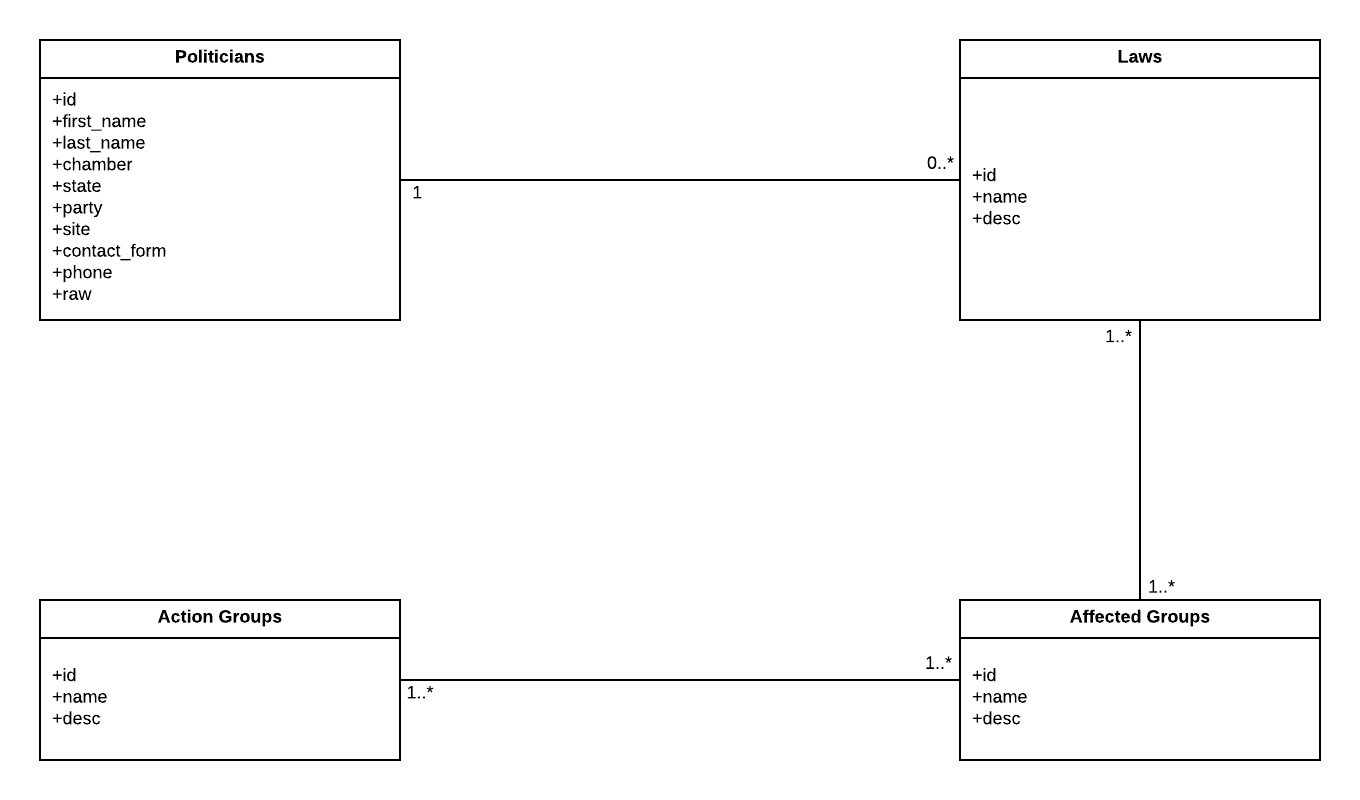
\includegraphics[width=\linewidth]{../Group8_UML.png}
%\end{figure}

\section{Testing}

We are using Selenium Python to test the GUI of our website. We installed Selenium with pip and downloaded the required interface driver for the Firefox browser (\code{geckodriver}), and then added \code{geckodriver.exe} in the system PATH. This let us use instances of Firefox WebDriver in our Python unit test to navigate around our website and test our GUI.
\\
\\
Since we are using Flask-Restless and SQLAlchemy to create our RESTFul API, we did not test our back-end because those tools handle it.
\\
\\
We are using Postman for API testing. The Postman test requests GET methods to our API and we make sure that all the fields we need in the database are present and have correct number of pages. 
\\
\\
We are using Mocha, Chai, and Enzyme to test our javascript. We installed Mocha, Chai, Enzyme, \code{babel-preset-env}, \code{babel-core}, \code{babel-preset-react}, and \code{react} in \code{npm} and ran \code{mocha} with arguments \code{--require babel-core/register}.

\section{Obstacles}
In Phase III of our IDB project we ran into a significant problem when we were trying to implement filter, sort and search. We had an issue with our code because of the way we set up our front-end in Phase I and Phase II and had to scrap much of the front-end code and refactor for Phase III. Although Phase III was supposed to be a lighter workload, this was not the case for us. We turned in our project a day late to ensure we had a working and well developed website.
\end{document}